\documentclass[Research_Module_ES.tex]{subfiles}
\begin{document}
\subsection{The Balanced Incomplete $CV(n_v)$}
Another version is the \textit{Balanced Incomplete CV($n_\nu$)}, denoted by $BICV(n_v)$. This variant uses only a subset $\mathcal{B}$ of the set of all possible partitions for a given $n_\nu$, which was given by $\mathcal{R}^\ast= \{s\subseteq\{1,\dots,n\}|\# s=n_v\}$. With $|\mathcal{B}|\equiv b$ as the number of partitions in the collection of partitions $\mathcal{B}$. This method does model selection by 
\begin{align*}
	BICV(n_\nu)=\min_{\alpha\in\mathcal{A}}\hat{\Gamma}_{\alpha,n}^{BICV}
\end{align*}
where $\hat{\Gamma}_{\alpha,n}^{BICV}$ is the estimator of the \textit{Expected Squared Prediction Error}. The structure of this estimator is the same as in Definition \ref{estimator CV(n_v)} by using the subset $\mathcal{B}$ instead of $\mathcal{R}^\ast$, thus the estimator has the following form
\begin{align*}
	\hat{\Gamma}_{\alpha,n}^{BICV}=|\mathcal{B}|^{-1}n_\nu^{-1}\sum_{s\in\mathcal{B}}\parallel y_s-\hat{y}_{\alpha,s^c}\parallel^2
\end{align*}
%Passive Voice
% and in the next step the reader will be introduced on how $BICV(n_v)$ chooses his partitions, namely by a combinatorical procedure such that the following \textit{balance conditions} hold.
Note that $\mathcal{B}$ is a \textit{balanced incomplete block design (BIBD)} of the set of validation data. We construct $\mathcal{B}$ as follows: 
\begin{defi}
\label{balance_property}
Let $\mathcal{B}$ be a collection of $b$ subsets of $\{ 1,\dots,n\}$ that have size $n_v$ such that the following two conditions hold:
\begin{enumerate}
\item[(a)] every $i$, $1\le i \le n$, appears in the same number of subsets of $\mathcal{B}$
\item[(b)] every pair $(i,j)$, $1\le i < j \le n$, appears in the same number of subsets of $\mathcal{B}$
\end{enumerate}
\end{defi}
The idea behind using \textit{BIBD}'s is to reduce the computational complexity of \textit{Cross-Validation}, hence $\mathcal{B}$ includes only a subset of the feasible partitions in $\mathcal{R}^\ast$. To avoid creating a bias, Definition \ref{balance_property} ensures that $\mathcal{B}$ has the same moment conditions as $\mathcal{R}^\ast$.
By choosing $b=O(n)$ we can show that $BICV(n_v)$ is asymptotically correct by the following theorem.\footnote{Proof of Theorem \ref{THM_Consistency_BICV} is given in Appendix \RM{1}}
\begin{thm}[Asymptotic Properties of $BICV(n_v)$]
	\label{THM_Consistency_BICV}
Under the conditions of Theorem \ref{THM_Consistency of $CV(1)$} and
\begin{align}
\lim_{n\to\infty} \max_{s\in \mathcal{B}}\biggl\lVert \frac{1}{n_v}\sum_{i\in s}x_ix_i' - \frac{1}{n-n_v}\sum_{i\in s^c}x_ix_i'\biggr\rVert =0. \label{gram_matrix_condition_BICV}
\end{align}
Suppose furthermore that $n_v$ is selected such that
\begin{align}
\frac{n_v}{n}\to 1 \quad \textrm{and} \quad n-n_v \to \infty. \label{growth_rates_nv_BICV}
\end{align}
Then the following holds
\begin{enumerate}[(I)]
\item If $\mathcal{M}_\alpha$ is in Category I, then there exist $R_n \ge 0$ such that $\hat{\Gamma}_{\alpha,n}^{BICV} = \frac{1}{n}\varepsilon'\varepsilon + \Delta_{\alpha,n} + R_n + o_P(1)$.
\item If $\mathcal{M}_\alpha$ is in Category II, then $\hat{\Gamma}_{\alpha,n}^{BICV} = \frac{1}{n}\varepsilon'\varepsilon + \frac{1}{n-n_v}d_\alpha\sigma^2  + o_P((n-n_v)^{-1})$.
\item $\lim_{n\to\infty}P(\mathcal{M}_{BICV}=\mathcal{M}_\ast) = 1$
\end{enumerate}
where $\mathcal{M}_{BICV}$ denotes the model selected by using $BICV(n_v)$.
\end{thm}
The most important difference between $CV(1)$ and the $BICV(n_\nu)$ is the choice of $n_\nu$. Assumption (\ref{growth_rates_nv_BICV}) implies that $n_\nu$ and $n$ grow with the same rate to infinity. Otherwise we end up asymptotically in the same case as in $CV(1)$.\\

Note, that $\hat{\Gamma}_{\alpha,n}^{BICV}\geq\Gamma_{\alpha,n}+o_p(1)$ for any $\mathcal{M}_\alpha\in$ Category I and that $\hat{\Gamma}_{\alpha,n}^{BICV}=\sigma^2+o_p(1)$ for any $\mathcal{M}_\alpha\in$ Category II. Together with Lemma \ref{Equation2.3-2.4} and (\ref{liminf_condition}), it follows that the $BICV(n_\nu)$ asymptotically picks models from Category II.\\

In general the validation sample $n_\nu$ should be selected relatively large in comparison to the construction data. Because if $n-n_\nu$ is large, then 
\begin{align*}
\hat{\Gamma}^{BICV}_{\alpha,n}=\sigma^2+\frac{1}{n-n_\nu}~d_\alpha\sigma^2+o_p\left(\frac{1}{n-n_\nu}\right)
\end{align*}
is flat such that it is difficult to find the minimum $\alpha$. But also we have to make sure that $n_\nu$ is not too large, since we need $n-n_\nu\to\infty$ to ensure the consistency of the OLS estimate.\\

The problem of flat functions is that  there is too much weight on the stochastic remainder terms such that \textit{Cross-Validation} can not correctly identify the minimum. Figure \ref{ProofSketchCV1} and \ref{ProofSektchCVn_v} show the \textit{Expected Squared Prediction Error} (dotted line) against their empirical counter part (solid lines) of two different Category II Models.\footnote{For more details, see simulation code Appendix II} As we can see in figure \ref{ProofSketchCV1} the error estimates are crossing each other. Every time they cross, the \textit{Cross-Validation} chooses the wrong model. Hence of the differences in scale, see figure \ref{ProofSektchCVn_v}, this problem does not occur that often for the $BICV(n_\nu)$.\\
\begin{figure}[!h]
	\label{ProofSketchCV1}
	\centering
	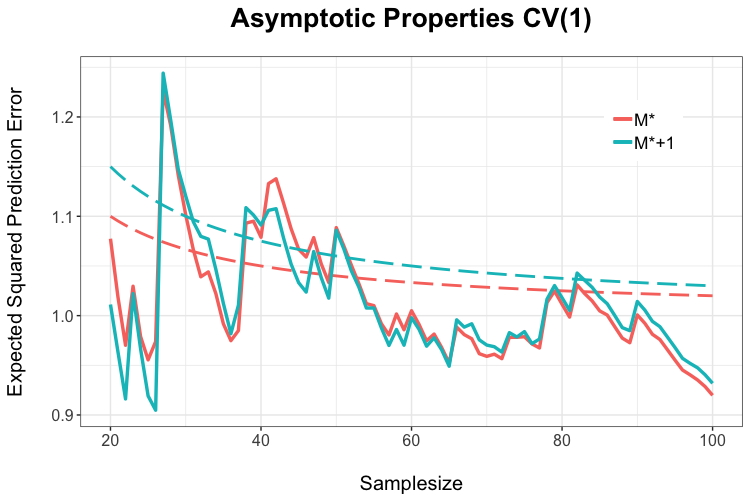
\includegraphics[width=0.8\textwidth]{ProofSketchN1.png}\\
	\caption{Estimated Squared Prediction Error $CV(1)$}
\end{figure}
\begin{figure}[!h]
	\label{ProofSektchCVn_v}
	\centering
	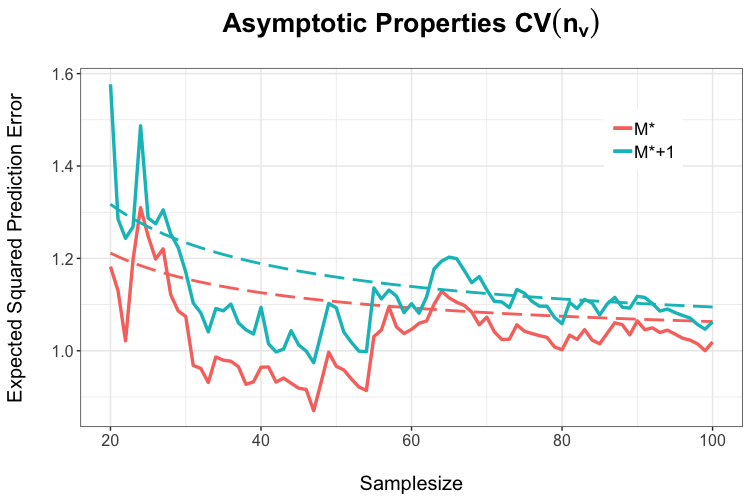
\includegraphics[width=0.8\textwidth]{ProofSketchNV.png}\\
	\caption{Estimated Squared Prediction Error $CV(n_\nu)$}
\end{figure}
\\
We need condition $\frac{n_v}{n}\to 1$ for the choice of $n_\nu$, because if this condition does not hold, $BICV(n_v)$ cannot distinguish in between the models in Category II and thus this method would be inconsistent (this is the main problem of CV(1) that occurs). For a more detailed explanation see \cite{shao}. We choose in our simulation $n_\nu=n-\lfloor n^{3/4}\rfloor$, which satisfy the above condition.\\

Note that condition (\ref{gram_matrix_condition_BICV}) is satisfied if the $x_i$ are iid random vectors, such that $E[(x_i^\prime x_i)^{2+\tau}]<\infty$ for some $\tau>7/3$.\footnote{See Claim \ref{Lala} in Appendix I}

%IRgendwie einen übergang und eine eiene Beschreibung schaffen(keine eigenen Worte, nur notizen hier benutzt und versucht zu sortieren)
%\textbf{NOTIZEN/Überlegungen}\\
%-explanation why $BICV(n_v)$ improves over CV(1):\\
%-$n_\nu$ should be choosen according to\\ \begin{align*}
%\frac{n_v}{n}\to 1 \quad \textrm{and} \quad n-n_v \to \infty.
%\end{align*}
%-need a large $n_\nu$ (for assessing the prediction ability) and a relative small $n-n_\nu$ (for construction data) because then
%\begin{align*}
%	\Gamma_{\alpha,n-n_\nu}=\sigma^2+(n-n_\nu)^{-1}d_\alpha\sigma^2
%\end{align*}
%is not a flat function and therefore it is easier to find a minimum of $\Gamma_{\alpha,n-n_\nu}$ for a small $n-n_\nu$\\
%-But the difference (that has to be small in comparison to the number of data used for validation) has to fullfill $n-n_v \to \infty$ to ensure the consistency of the model fit\\
%-Need condition $\frac{n_v}{n}\to 1$ for the choice of $n_\nu$, because if this condition does not hold, $BICV(n_v)$ cannot distinguish in between the models in Category II and thus this method would be inconsistent (This is the main problem of CV(1) that occurs)\\
%ICh denke das ist gemeint beim teleskop argument, BICV ist fähiger die unterschiede besser zu erkennen, also unter gegebenen umständen kann es sogar innerhalb der cat2 models unterscheiden, was cv1 einfach nicht kann- so habe ich es verstanden, damit ist die vorhersagegenauigkeit einfach besser bei bicv als bei cv1 (also bicv erkennt unterschiede noch besser als cv1 und gewährt somit eine bessere modelselection)
%-As we have seen, CV(1) is asymptotically inconsistent, it cannot distinugish in between category II models; if we choose $n_\nu$ such that these two conditions for $n_\nu$ in Theorem \ref{THM_Consistency_BICV} do hold, then $BICV(n_v)$ improves over CV(1) because it is able to distinguish and consistent

\end{document}